\documentclass[12pt, ]{scrartcl}
\usepackage[style=alphabetic]{biblatex}
\usepackage{graphicx}
\graphicspath{{./graphics}}
\addbibresource{bibliography.bib}
\usepackage{multicol}
\usepackage{setspace}
%opening
\title{Improvement of the Bayesian generalization model in order to handle negative examples and discontinuous hypotheses}

\begin{document}
\def\isblind{1}
\if\isblind0
    \author{Jason Cramer, Maximilian Dierschke, Nils Engleder}\fi
\if \isblind1
    \author{}\fi

\maketitle
\begin{abstract}
	abstract-text
\end{abstract}
\doublespacing
\begin{multicols}{2}
\section{Background}
The problem our project is focusing on is Shepard's ideal generalization problem. The generalization problem focuses on how humans build hypothesis spaces for a given consequence after observing stimuli.
In the paper "Generalization, similarity, and bayesian inference", they discuss how using a model of bayesian inference, we can predict the probability of given stimuli being included within the consequential region \cite{Tenenbaum}.
The model uses the equation $p(y \in C \mid x) = \sum\limits_{h:y\in h} p(h | x)$ where $h$ is a hypothesis from the hypothesis space ${\cal H}$ and $p(h | x)$ is the posterior probability of  the hypothesis after observing x.
We plan to extend this model to investigate how including negative examples within the x vector(x is the observed stimuli) affect how the model limits hypotheses. We also plan to explore how different distributions and models compare to the original model for generalization.
\section{Question}
To generalize the model by Tenenbaum et al, we want to find a way, how it can be improved, so that it can handle negative examples and discontinuous hypotheses.

\section{Negative examples in the baseline model}
The baseline model (Figure \ref{fig:baseline}), which was introduced by Tenenbaum et al. is by itself not capable of handling negative examples.

\begin{figure}[t]
	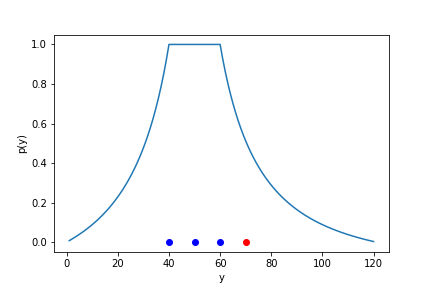
\includegraphics[width=4cm]{graphics/baseline.png}
	\centering
	\caption{Baseline model fitted on the positive examples [40, 50, 60] (red) does not incorporate the negative examples (70,80) }
	\label{fig:baseline}
\end{figure}

A naive approach to incorporate negative examples, is to fit a model the same way it was fitted for the positive examples and then  calculate the difference.

\noindent

Evaluate how negative examples affect the predictions of the original model and use it as a baseline
(2) Evaluate the predictions made by the original model for multi cluster sample data
\section{multi cluster sample data}
(3) Evaluate how the model could be altered so that negative examples can be incorporated to limit cluster intervals assuming a continuous consequential region
\section{multi}
(4) Evaluate how the model could be altered so that negative examples can be incorporated to limit cluster intervals assuming a discontinuous consequential region
1
(5) Evaluate how the model can be expanded to handle discontinuous regions without
negative examples
We want to initially solve the first three issues. Due to the added co

We start with a naive approach, where we will use the base model and fit one to positive and one to negative examples.

\centering

\nocite{*}
\printbibliography
\end{multicols}
\end{document}
